\graphicspath{{Images/conclusion/}}

\chapter{conclusions and future work}
\label{chap:conclusion}
This Ph.D. research is performed as part of office of the naval research (ONR) funded project titled `Octopus-Inspired Autonomous Arms for Soft Robotics with Adaptive Motions'. The team consisted of roboticists, material scientists, and controls engineers conducted research on multiple disciplines simultaneously, which helped the informed progress of one field by considering the requirements of the other. This unique combination resulted in solving some of the key technical challenges ahead of soft robotics in general and of miniature, untethered soft robots in particular. Also, this research have some broader impact on soft robotics community and can change the way the robots are created in the future which will be discussed in this chapter.
\section{Technical and Scientific Impact}
The technical contribution of this dissertation in material science can be explained as improving the performance of PNIPAAm-based hydrogels to make them usable in soft robotic systems. These improvements include:
\begin{itemize}
 \item Increasing the speed of the hydrogel's response to the temperature changes. Prior to this improvement, the gel response was slow and therefore, no meaningful robotic movement was produced in reasonable amount of time. 
 \item Using a synthesis technique based on photopolymerization to minimize the polymerization time (to under 15 sec) and facilitate the fabrication of hydrogel structures. Prior research focused on improving the response rate without considering the ease of manufacturing and therefore the resulting gels were of less interest in the robotics community.
 \item Expanding the knowledge on underlying the mechanisms of transport phenomena in temperature-responsive hydrogles as well as the effect of their micro-structure on their response. 
 \item Expanding the knowledge on the mechanism of pore formation in hydrogels based on non cononsolvency effect. 
 \item Studying the tunability of the response of the hydrogels based on simple tweaking of ingredients. 
\end{itemize}
	
In terms of manufacturing, a bottom-up assembly approach inspired by biology has been selected to facilitate the fabrication of soft robots. Using building blocks to assemble soft robots. Building blocks can be selected from a wide range of materials. They can also contain essential components such as sensors and processors. The manufacturing of a building block is very simple and therefore they can be mass produced easily. These features facilitates the fabrication of multimaterial structures. This is critical while the range of compatible materials for 3D printing is still limited.  Inclusion of electronics in the soft robot structure would also be performed more easily.  
\subsection{Broader Impact on Soft Robotics Community}
Soft robotics has quickly turned into a broad area of research since its introduction. Therefore, new challenges have already been raised and more will be faced in the future. One of these challenges is to cut the tether from robots and enable them to operate as mobile devices. Another challenge is to reduce the size of the robots. An even tougher problem would arise when trying to solve both the aforementioned challenges simultaneously. Addressing these challenges require innovative approaches and usually requires progress in multiple fields. However, often the progress in one field is made without considering the limitations of the other fields. This problem is more profound in the field of material science regarding the development on novel materials for soft actuators and sensors. For instance, stimuli-responsive hydrogels are usually developed using complex processes and specialized equipment and therefore they are less accessible to robotics community. 

Within the field of heterogeneous hydrogel structures, the presented methods in material synthesis and manufacturing techniques have helped to achieve unique desirable features that are highly demanded in hydrogels and soft robotics research simultaneously. In the literature surveyed, individual features might have been achieved separately. However, since some of the goals are counteracting, reaching one makes the other harder to achieve. For example, improving the response rate of hydrogels is highly regarded from a materials research perspective but is often accompanied by complications in synthesis which is less favorable from a manufacturing point of view. Parallel improvements have been made through a collaboration between teams of material scientists and roboticists allowing considerations from one field to inform the other.  

In addition, by introducing the first addressable hydrogel voxels,  the field is further advanced by creating on-demand actuation and shape change of heterogeneous structures --a feature that improves the motion of a structure from hard-coded to on-demand programmable. As mentioned above, on-demand programmable shape change is one of the main goals of research in this field which is hard to achieve using the current technologies. It should be emphasized that the control signals are electrical signals, a feature inspired by biology in contrast to the previously demonstrated heterogeneous structures which use light signals or global temperature changes. Therefore, the robotic systems can be miniaturized and fully untethered simultaneously.
\subsection{Broader Impact on Society}
This research on soft robotics have many potential applications in biology, medicine and environmental science. The small footprint soft robots developed are low cost and can be manufactured in large numbers. A swarm of these robots can operate under water to collect environmental data, thanks to the intrinsic compatibility of hydrogels and water. The miniature robots can be sent inside the human body to perform drug delivery, biopsies, and tasks that require a high number of degrees of freedom in robotic manipulators.
In addition to the capability of soft robots in dealing with unstructured environment, they are intrinsically safe around humans. This can enhance the application of robots to daily life uses such as household robots and assistant robots for elderly people which are challenging using rigid robots.
\section{Future Work}
The research presented in this dissertation has opened the doors to a variety of other research opportunities. Some of these new research in the field of control of soft robots and in-depth analysis of the hydrogel materials  have already been started by different teams consisting of Ph.D., Masters and undergraduate students. An introduction to these work will be presented here and future opportunities will be discussed.
\subsection{In-depth analysis of noncosolvencey phenomenon}
While the research in this dissertation provides a method of altering the properties of  temperature-responsive PNIMPAAm hydrogels by means of mixed solvent method, the mechanisms of pore formation in this method is not fully understood. To study these mechanisms, our collaborators in the University of California, Los Angeles (UCLA) have started in-depth study of the hydrogels produced by the mixed solvent method. It is understood that the coil to globule transition of polymer chains in presence of a second solvent (Figure~\ref{fig:cononsolv}) results in the formation of pores. 
\begin{figure}[!ht]
\centering
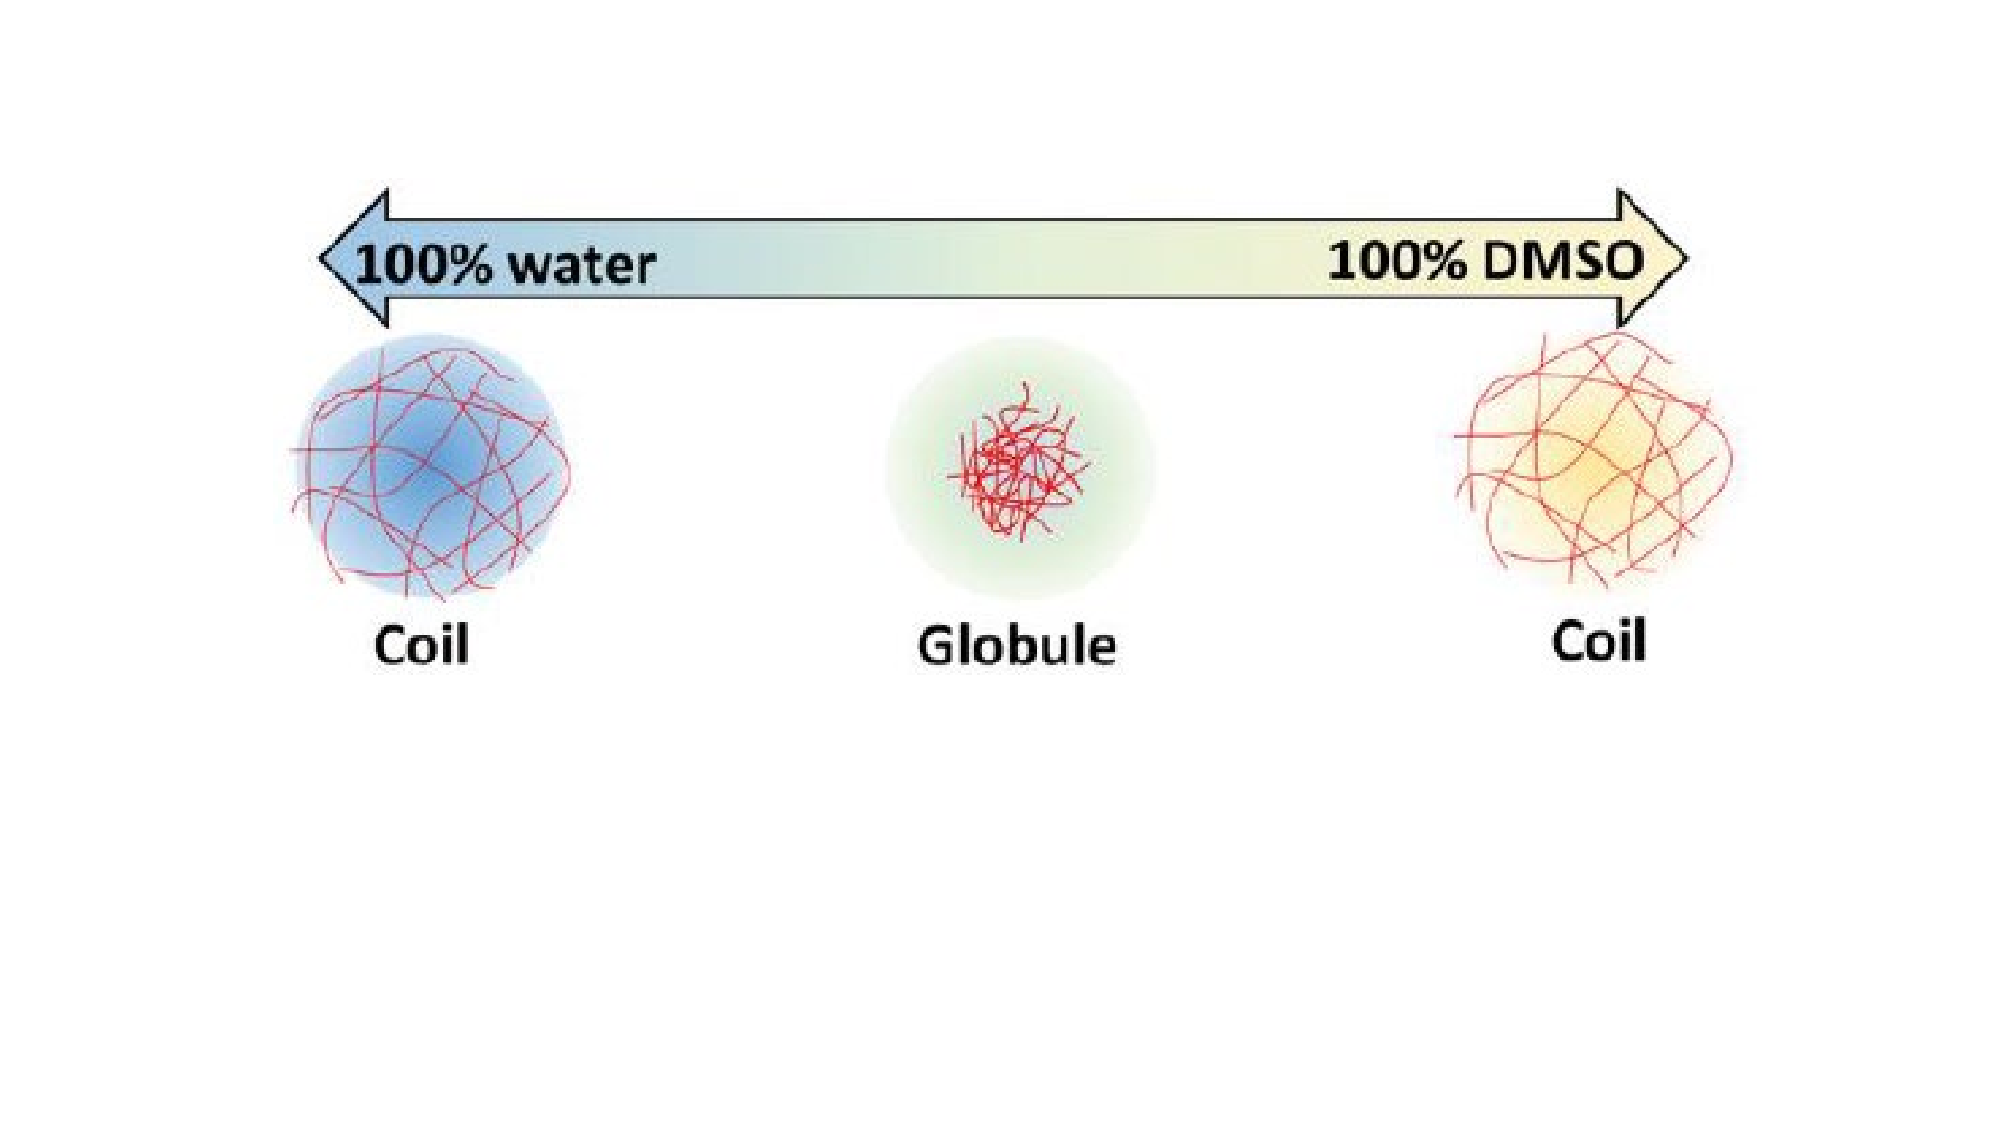
\includegraphics[width=0.7\textwidth]{cononsolv.pdf}
    \caption[]{}
    \label{fig:cononsolv}
\end{figure}

In addition, a 3D printing technique has been demonstrated. A sample 3D printed structure is shown in Figure~\ref{fig:3Dprint}. The results of this research has been accepted for publication in Advanced Materials Journal. Future work will focus on 3D printing of voxels with embedded soft heaters to remove the rigid components from the voxels and increase their production rate.
\begin{figure}[!ht]
\centering
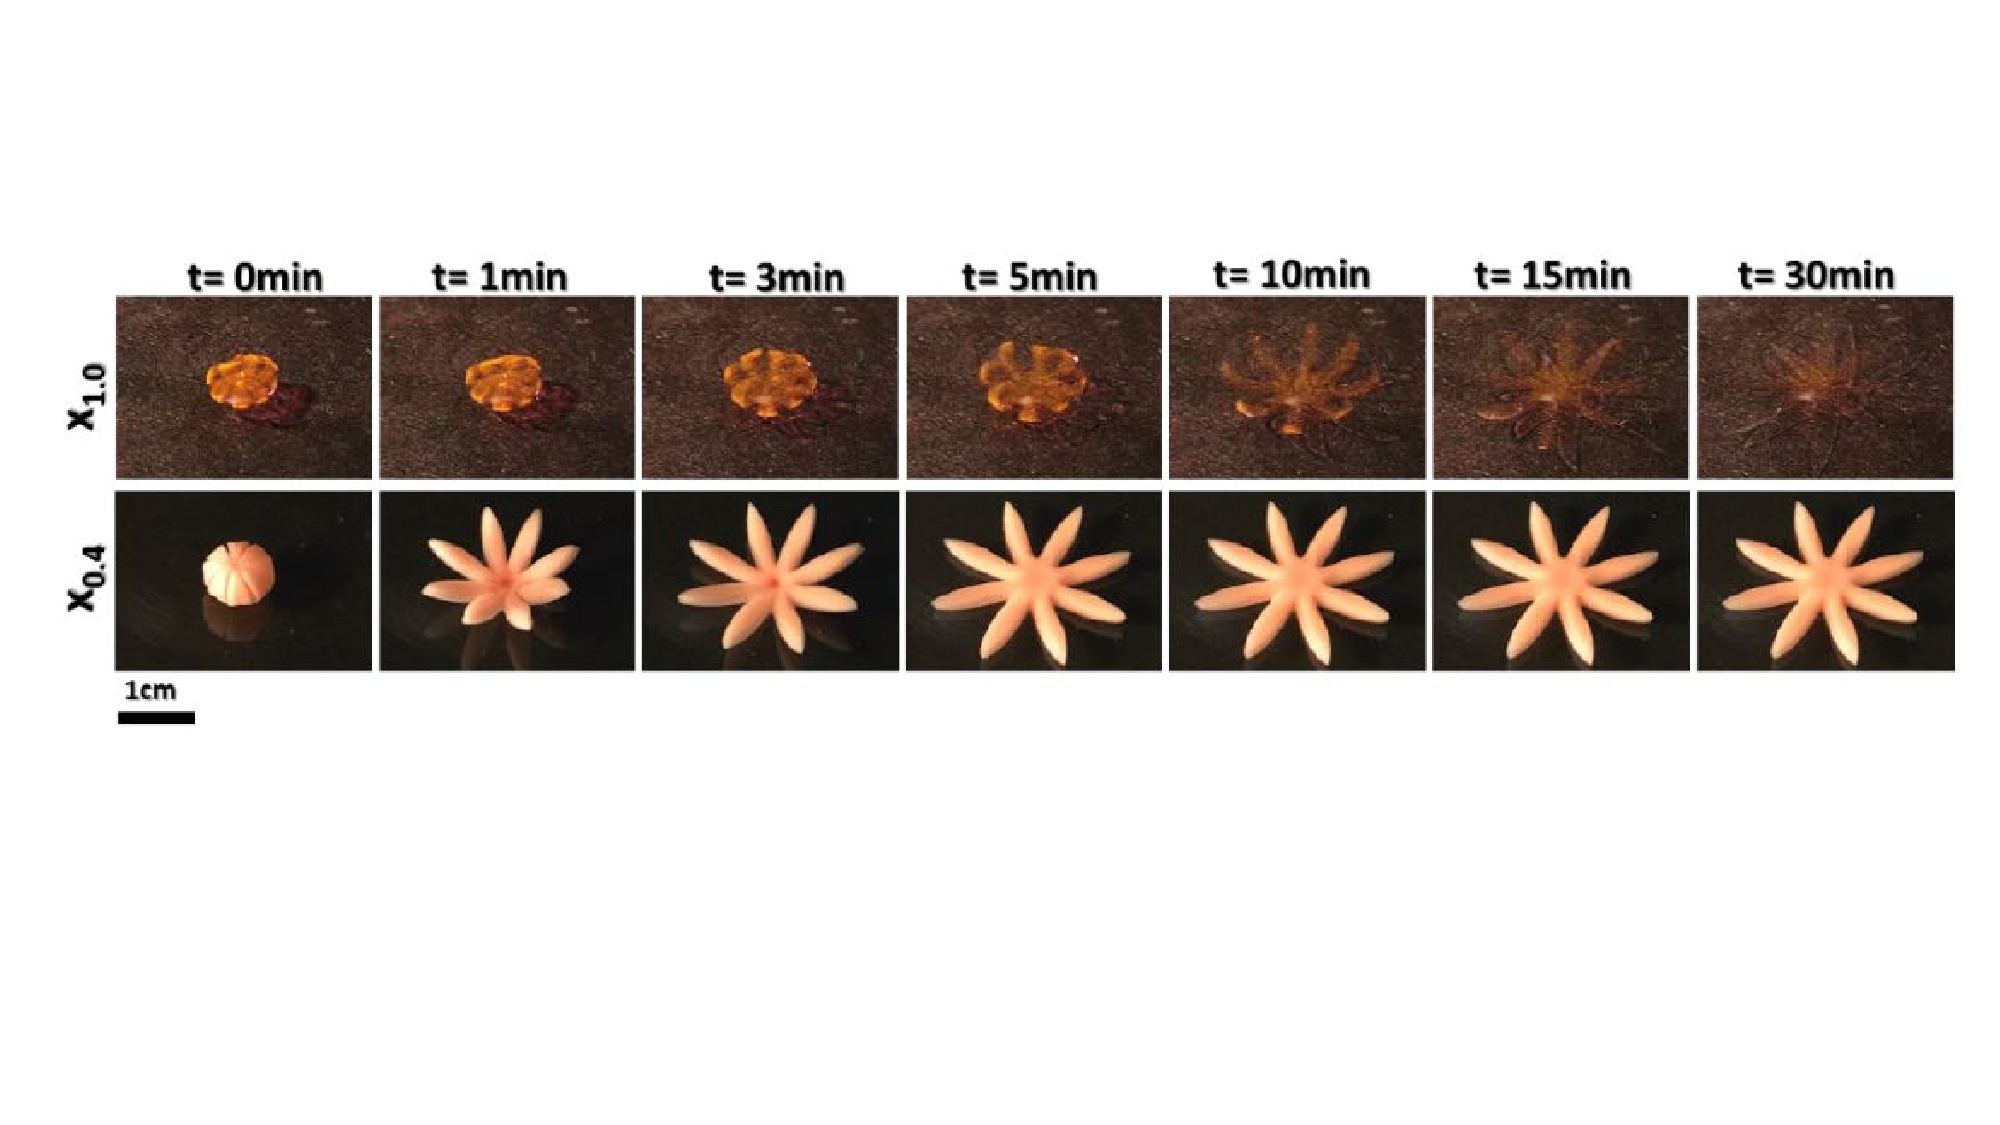
\includegraphics[width=\textwidth]{3Dprint.pdf}
    \caption[]{}
    \label{fig:3Dprint}
\end{figure}

\subsection{Control of the Hyper-redundant Robotic Arm}
The electrical stimulation of SVAs helps the control engineers to implement and test their algorithm on the developed robot prototypes. In \ref{chap:control} we have discussed the an example of such controller in a mechanism consisting of two SVAs. More complex structures such as the 16 DOF miniature manipulator discussed in \ref{chap:heterogeneous} can also be controlled on the same basis which is discussed in a more recent work~\cite{Doroudchi2020}. 
So far, all the sensing required for the closed-loop control was performed using a camera. For embedded system it is essential that the sensors are included in the robot. Future work includes finding sensor solutions that can detect the motion of the robot and can be embedded in the robot. 
%\begin{figure}[!t]
%\centering
%\includegraphics[width=0.7\textwidth]{control.pdf}
    %\caption[]{}
    %\label{fig:control}
%\end{figure}

%\subsection{Finite Element Modeling of the Hydrogel Structures}
%\begin{figure}[!t]
%\centering
%\includegraphics[width=0.7\textwidth]{FEM.pdf}
    %\caption[]{}
    %\label{fig:FEM}
%\end{figure}

\subsection{Dynamic Simulation of the Voxel-based Robots}
While the finite element modeling provides accurate information about the deformation of the hydrogels considering the details of the transport of water in the porous structures, the time required for such simulations are usually long. For soft robot prototyping, it is essential to have tools that can predict the motion of the robot and provide insight about the performance of a particular design. Different tools have been developed for this purpose such as SOFA~\cite{} which uses a hybrid FEM and lumped model engine and VoxCAD~\cite{} which is based on a voxel-based, mass-spring lattice modeling. Work is in progress to expand the possibilities of VoxCAD by adding functionalities such as controlling individual voxel deformation instead of a global deformation function. An example gripper is shown in Figure~\ref{fig:voxcad}
\begin{figure}[!t]
\centering
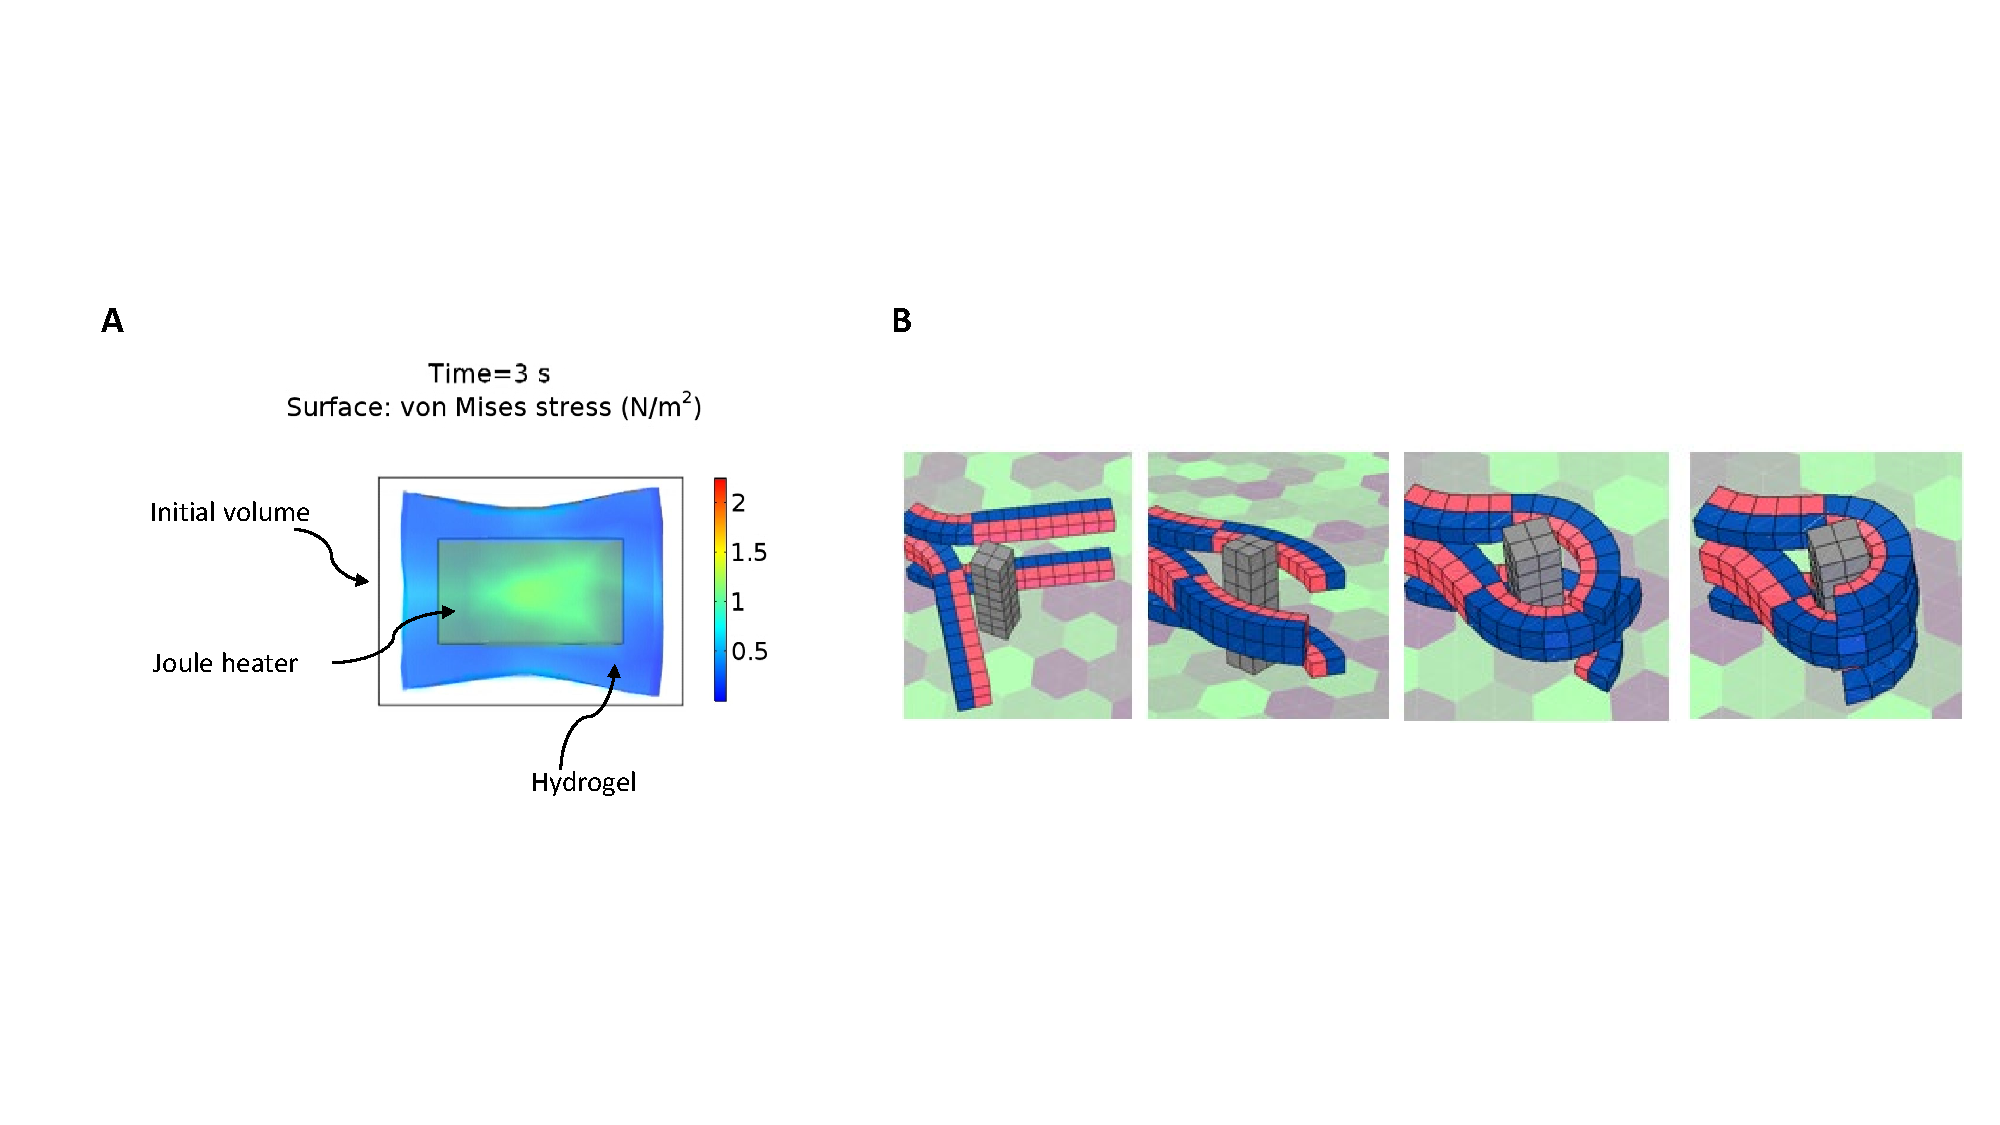
\includegraphics[width=\textwidth]{voxcad.pdf}
    \caption[Dynamic simulations]{Dynamic simulations using FEM and mass-spring methods. A) FEM simulation of a voxel contraction as the Joule heater is turned using COMSOL. B) Mass-spring model simulation of a gripper using a modified version of VoxCAD. }
    \label{fig:voxcad}
\end{figure}

\subsection{A 3-dimensional prototype of the hyper-redundant robot}
Extending the motion of the miniature hyper-redundant arm discussed in \ref{chap:heterogeneous} to 3D is the next step in the development of this arm. Also this next version would be modular such that different arm segments can be attached together to achieve more complex robots. Each segment has its own computation power, sensors and power supply making it completely independent of other segments. Also each segment can communicate with other segments to perform a shared goal. This prototype can help control engineers to explore the distributed sensing and control algorithms inspired by octopus where some of the control task is not performed by a central nervous system but by a distributed neural network across its arms. A schematic of the idea of a 3D segmented arm is shown in Figure~\ref{fig:3Darm}
\begin{figure}[!t]
\centering
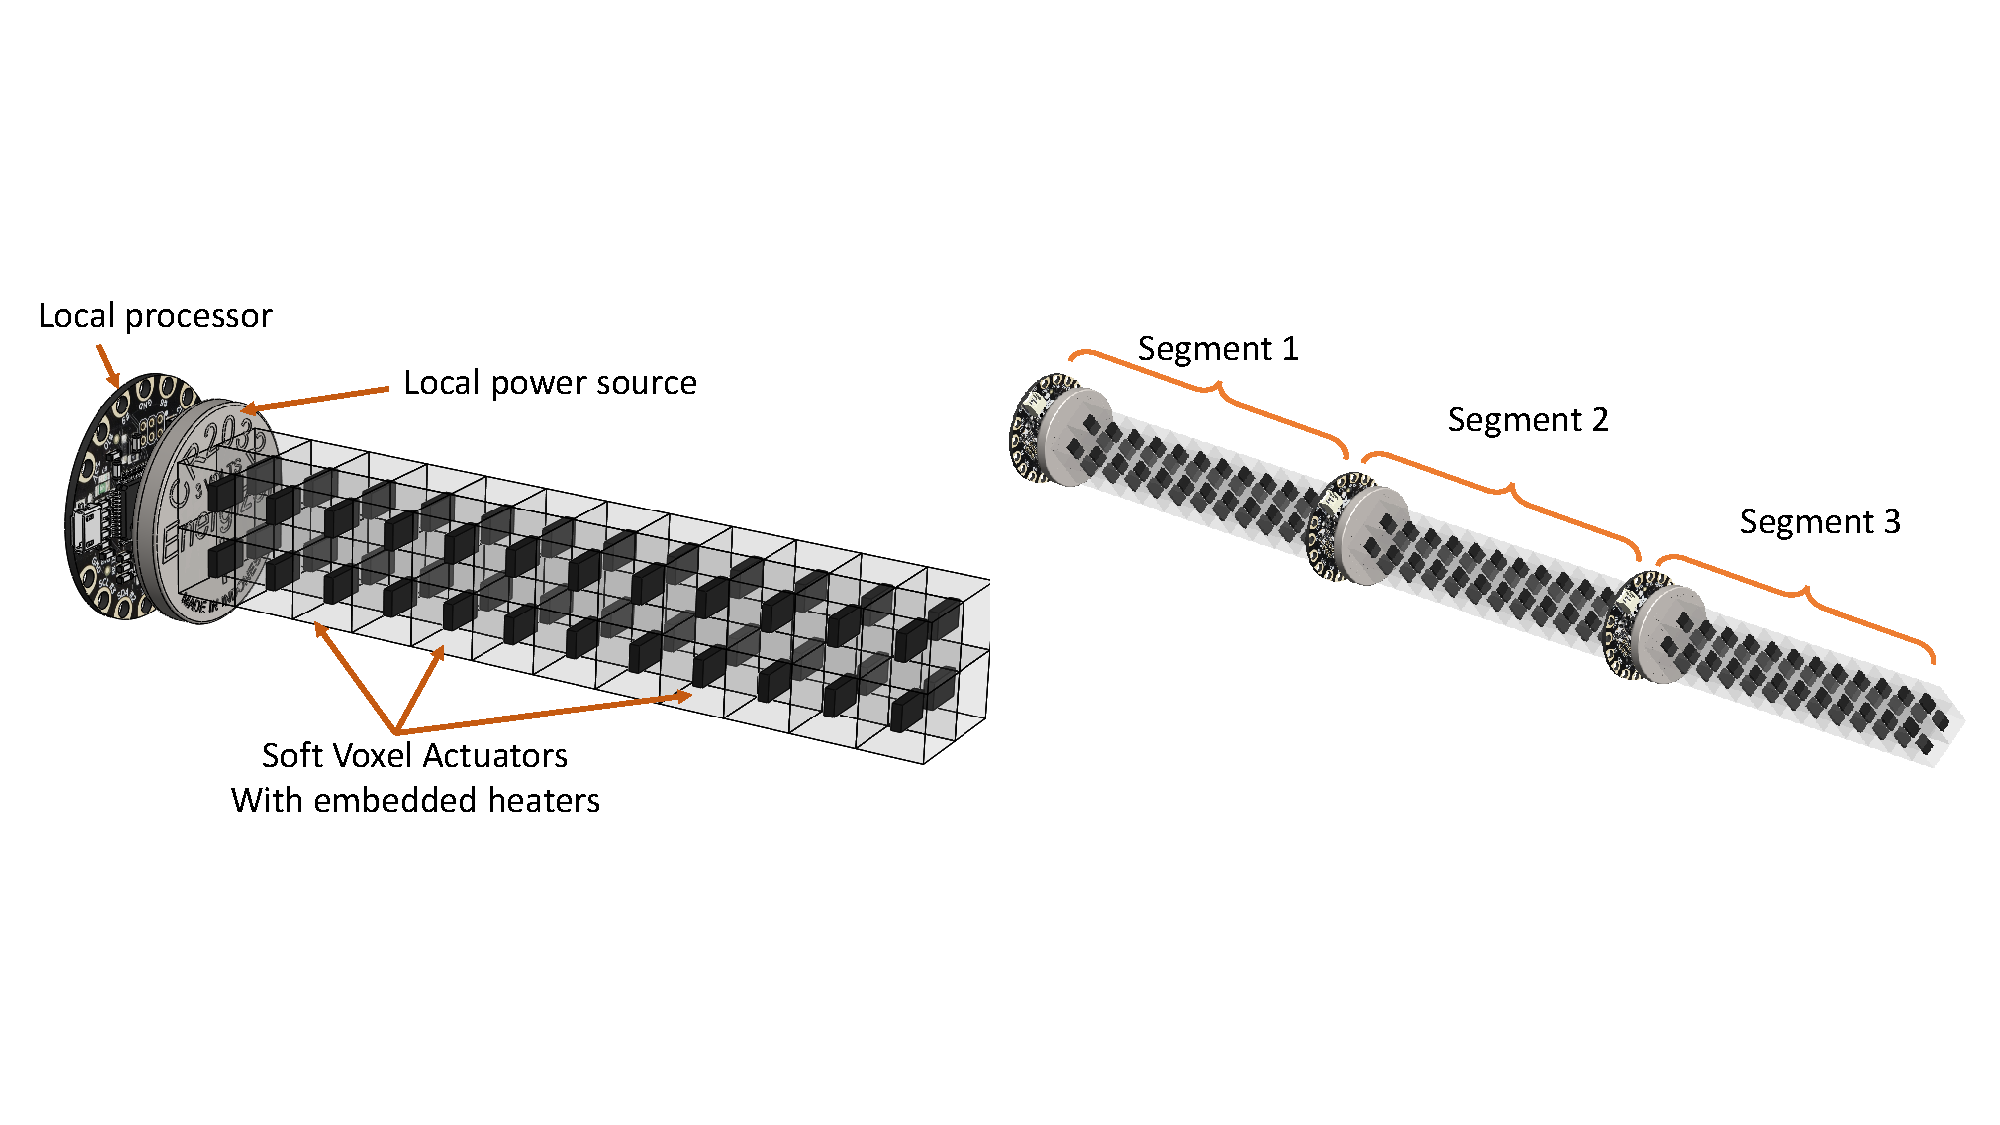
\includegraphics[width=\textwidth]{3Darm.pdf}
    \caption[3-dimensional miniature arm]{The concept of a 3-dimensional miniature arm segment with embedded power and processor (left). An assembly of segments forming a more complex arm (right)}
    \label{fig:3Darm}
\end{figure}

\subsection{Expanding the Functionality of the Robots}
It is widely accepted that the soft robot can outperform rigid robots in terms of adaptability. For example, a robot that needs to be at a certain size for performing its routine tasks, but should be able to reduce its size for squeezing into tight spaces can be made out of soft materials in theory. In practice however, the limitations such as controlling the soft robots and embedding efficient sensors for feedback have so far prevented the demonstration of such tasks by soft robots. These challenges are known to soft robotics community and there has been increasing effort in addressing them. For instance, the relatively new IEEE soft robotics conference (RoboSoft) has started a robotic competition the goal of which is to invite the community to solve some of the mentioned challenges. Figure~\ref{fig:sorocomp} shows the schematic of the competition goals, setup and requirements. Making soft robots using SVAs that can perform some of the tasks mentioned in Figure~\ref{fig:sorocomp} is one of the routes to follow in the future towards more impactful soft robots that can deal with real world situations. 
\begin{figure}[!t]
\centering
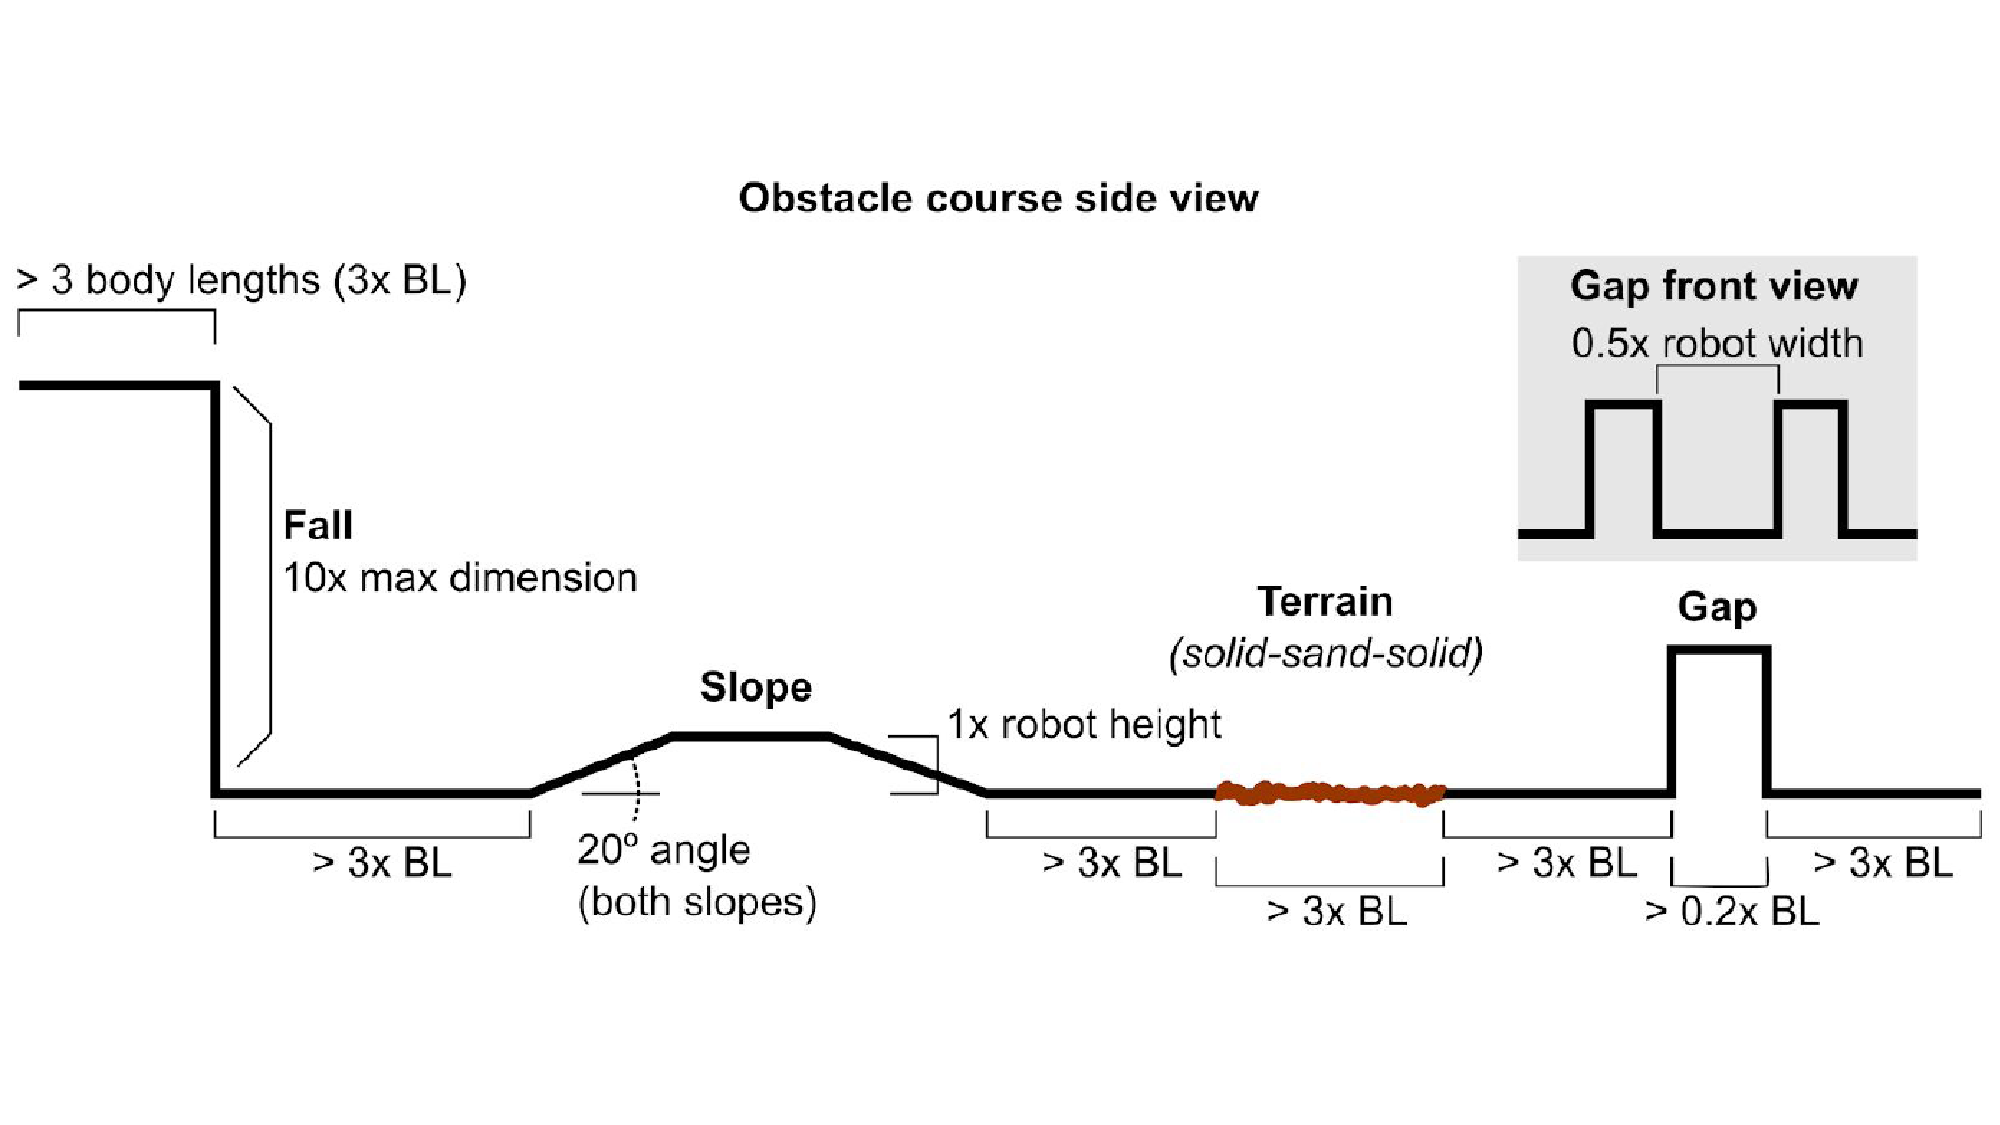
\includegraphics[width=0.8\textwidth]{sorocomp.pdf}
    \caption[SoRo robotic competition]{Schematic showing the requirements, setup and goals in robotic competition as part of IEEE RoboSoft conference.}
    \label{fig:sorocomp}
\end{figure}

\subsection{Untethered Octopus Inspired Robot}
The miniature continuum manipulators can be assembled into more complex robots as shown in Figure~\ref{}. These robots can operate autonomously and communicate through the built in wireless communication hardware. Regaring the low production cost, a swarm of these robots can be produced and be used for data collection and monitoring of environmental conditions. 
\begin{figure}[!t]
\centering
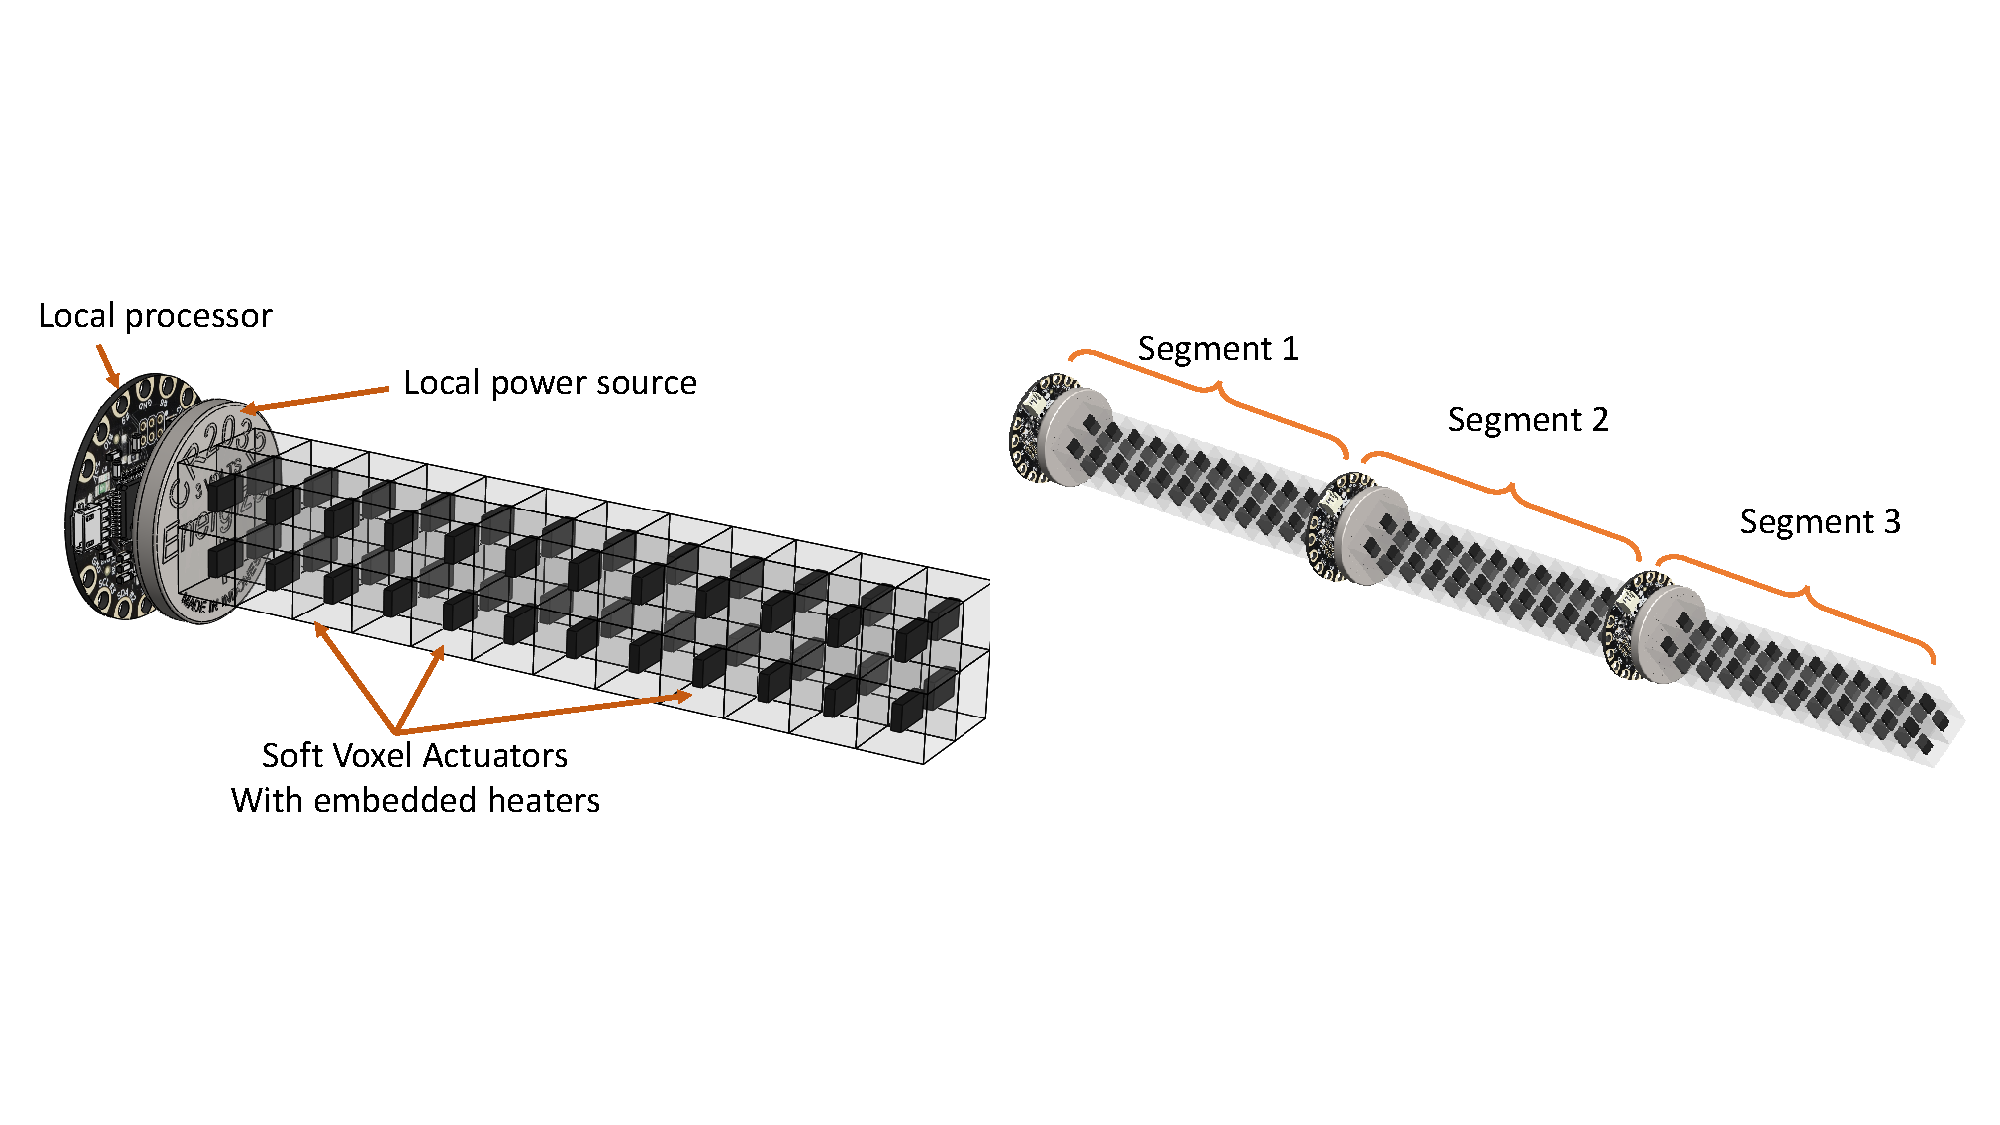
\includegraphics[width=\textwidth]{3Darm.pdf}
    \caption[3-dimensional miniature arm]{The concept of a 3-dimensional miniature arm segment with embedded power and processor (left). An assembly of segments forming a more complex arm (right)}
    \label{fig:3Darm}
\end{figure}
